\documentclass[12pt]{report}
\usepackage[fontsize=13pt]{scrextend}
\usepackage[utf8]{vietnam}
\usepackage[utf8]{inputenc}
\usepackage[vietnamese]{babel}
\usepackage{titlesec}
\usepackage{titletoc}
\usepackage{listings}
\usepackage[bookmarks=true]{hyperref}
\usepackage[left=3cm,right=2cm,top=2.5cm,bottom=3cm]{geometry}
\usepackage{graphicx}
\usepackage{hyperref}
\usepackage{tikz}
\usepackage{varwidth}
\usepackage{float}
\usepackage{listings}
\usepackage{color}
\usepackage{multirow}
\usepackage{booktabs}
\usepackage[ruled,vlined]{algorithm2e}

\setlength{\parskip}{6pt}

\usetikzlibrary{calc}
\setlength{\parindent}{10mm}
\renewcommand{\baselinestretch}{1.3}
\graphicspath{{images/}}

\definecolor{dkgreen}{rgb}{0,0.6,0}
\definecolor{gray}{rgb}{0.5,0.5,0.5}
\definecolor{mauve}{rgb}{0.58,0,0.82}

% setup code area as listings
\lstset{frame=tb,
  language=Java,
  aboveskip=3mm,
  belowskip=3mm,
  showstringspaces=false,
  columns=flexible,
  basicstyle={\small\ttfamily},
  numbers=left,
  numberstyle=\tiny\color{gray},
  keywordstyle=\color{blue},
  commentstyle=\color{dkgreen},
  stringstyle=\color{mauve},
  breaklines=true,
  breakatwhitespace=true,
  tabsize=3
}
\renewcommand{\lstlistingname}{Mã nguồn}
\newenvironment{thuattoan}[1][h]
  {\renewcommand{\algorithmcfname}{Thuật toán}
   \begin{algorithm}[#1]
  }{\end{algorithm}}

% hyper setup
\hypersetup{
	bookmarks=true,
	pdftitle={Xây dựng công cụ hỗ trợ quản lý và đảm bảo chất lượng cho các phiên bản phần mềm},
	pdfauthor={Bùi Quang Cường}, % author
	pdfsubject={TeX and LaTeX},
	pdfkeywords={TeX, LaTeX, graphics, images}, % list of keywords
	colorlinks=true,       % false: boxed links; true: colored links
	linkcolor=blue,       % color of internal links
	citecolor=black,       % color of links to bibliography
	filecolor=black,        % color of file links
	urlcolor=purple,        % color of external links
	linktoc=page            % only page is linked
}

\date{}


\newpagestyle{long}
{\sethead{\thesection. \sectiontitle}{}{\subsectiontitle}\headrule
	\setfoot{}{\thepage}{}}

\begin{document}
\begin{titlepage}
	\center
	\begin{tikzpicture}[overlay,remember picture]
		\draw [line width=3pt,rounded corners=0pt,]
		($ (current page.north west) + (25mm,-25mm) $)
		rectangle
		($ (current page.south east) + (-15mm,25mm) $);
		\draw [line width=1pt,rounded corners=0pt]
		($ (current page.north west) + (26.5mm,-26.5mm) $)
		rectangle
		($ (current page.south east) + (-16.5mm,26.5mm) $);
	\end{tikzpicture}
	
	{\large \bfseries ĐẠI HỌC QUỐC GIA HÀ NỘI\\ TRƯỜNG ĐẠI HỌC CÔNG NGHỆ}\\[1cm]
	
\includegraphics[width=0.2\linewidth]{uet}\\[1cm]
	{\Large  \bfseries Bùi Quang Cường}\\[1.5cm]
	{ \LARGE \bfseries XÂY DỰNG CÔNG CỤ HỖ TRỢ QUẢN LÝ VÀ ĐẢM BẢO CHẤT LƯỢNG CHO CÁC PHIÊN BẢN PHẦN MỀM}\\[0.5cm]
	\hfill\\[1.5cm]
	{\large \bfseries KHÓA LUẬN TỐT NGHIỆP ĐẠI HỌC HỆ CHÍNH QUY}\\	
	{\large \bfseries Ngành: Công nghệ thông tin}	
	\hfill\\[3.5cm]	
	{\large \bfseries HÀ NỘI - 2018}\\	
	\vfill
\end{titlepage}
	
%-----SECONDARY TITLE PAGE-----%	
\begin{titlepage}
	\center
	\begin{tikzpicture}[overlay,remember picture]
		\draw [line width=3pt,rounded corners=0pt,]
		($ (current page.north west) + (25mm,-25mm) $)
		rectangle
		($ (current page.south east) + (-15mm,25mm) $);
		\draw [line width=1pt,rounded corners=0pt]
		($ (current page.north west) + (26.5mm,-26.5mm) $)
		rectangle
		($ (current page.south east) + (-16.5mm,26.5mm) $);
	\end{tikzpicture}
	
	{\large \bfseries ĐẠI HỌC QUỐC GIA HÀ NỘI\\ TRƯỜNG ĐẠI HỌC CÔNG NGHỆ}\\[2cm]

	{\Large  \bfseries Bùi Quang Cường}\\[2cm]		
	{ \LARGE \bfseries XÂY DỰNG CÔNG CỤ HỖ TRỢ QUẢN LÝ VÀ ĐẢM BẢO CHẤT LƯỢNG CHO CÁC PHIÊN BẢN PHẦN MỀM}\\[0.5cm]
	\hfill\\[1.5cm]
	{\large \bfseries KHÓA LUẬN TỐT NGHIỆP ĐẠI HỌC HỆ CHÍNH QUY}\\	
	{\large \bfseries Ngành: Công nghệ thông tin}
	\hfill\\[2cm]
	\begin{flushleft}
		{\large \bfseries Cán bộ hướng dẫn: PGS. TS. Phạm Ngọc Hùng}\\	
	\end{flushleft}
	\hfill\\[3cm]		
	{\large \bfseries HÀ NỘI - 2018}\\		
	\vfill		
\end{titlepage}

%-----THANKS-----%
\newpage
\begin{titlepage}
\begin{center}
	\textbf{\large LỜI CẢM ƠN}
\end{center}
Đầu tiên, tôi xin gửi lời cảm ơn chân thành và sâu sắc tới thầy giáo PGS. TS. Phạm Ngọc Hùng – người đã trực tiếp hướng dẫn tận tình và đóng góp những ý kiến quý báu trong suốt quá trình tôi học tập, nghiên cứu cũng như khi tôi làm khóa luận tốt nghiệp này, người đã cho tôi nhiều lời động viên, những kiến thức quý báu giúp tôi trưởng thành hơn trong cuộc sống.

Tôi xin gửi lời cảm ơn tới những người bạn trong tập thể K59CLC – những người đã luôn đồng hành cùng tôi suốt bốn năm qua trên mọi nẻo đường, giúp đỡ tôi mỗi khi khó khăn, chia sẻ cùng tôi mọi chuyện trong học tập và cuộc sống và góp ý cho tôi những lời khuyên chân thành giúp tôi học tập tốt hơn và hoàn thành khóa luận này.

Tiếp theo tôi xin gửi lời cảm ơn đến các thầy cô giảng viên Trường Đại học Công Nghệ - Đại Học Quốc Gia Hà Nội – những người đã tận tâm truyền đạt những kiến thức quý báu làm nền tảng để tôi tiếp tục đi xa hơn nữa trong lĩnh vực công nghệ thông tin.Cuối cùng, tôi xin được cảm ơn cha mẹ, anh chị và người thân, những người đã không quản khó khăn, vất vả nuôi con ăn học để con có thể phấn đấu trở thành người có ích cho xã hội.
\end{titlepage}

	
%-----ABSTRACT-----%
\newpage
\begin{titlepage}
\begin{center}
	\textbf{\large TÓM TẮT}
\end{center}
\textbf{Tóm tắt:} Mã nguồn ứng dụng trở nên lớn và phức tạp sau quá trình dài phát triển, bảo trì và nâng cấp. Vấn đề này đang dần phổ biến đối với các doanh nghiệp phát triển phần mềm, gây khó khăn trong việc kiểm soát và đảm bảo chất lượng cho các ứng dụng. Hiện nay đã có một số công cụ được đề xuất để giải quyết vấn đề trên nhưng chưa có kết quả thỏa đáng. Nghiên cứu này đề xuất các phương pháp và xây dựng một bộ công cụ toàn diện cho việc phân tích và đảm bảo chất lượng mã nguồn cho các ứng dụng doanh nghiệp sử dụng các nền tảng J2EE phổ biến Struts 2, Hibernate, Spring. Đầu tiên, mã nguồn của ứng dụng sẽ được tiền xử lý để tạo cây cấu trúc. Mỗi nút trên cây đại diện cho một thành phần mã nguồn. Tiếp theo, các nút sẽ được phân tích theo các công nghệ sử dụng trong ứng dụng để xác định mối quan hệ phụ thuộc. Cây cấu trúc này được sử dụng làm đầu vào cho việc phân tích ảnh hưởng sự thay đổi và các chức năng phân tích cấu trúc như xây dựng đồ thị dữ liệu; xây dựng kiến trúc về công nghệ, cơ sở dữ liệu; tính toán độ phức tạp mã nguồn. Phương pháp phân tích ảnh hưởng sự thay đổi được đề xuất cải tiến theo hướng tự động hóa bằng phương pháp so sánh các phiên bản mã nguồn. Hiện nay, bộ công cụ đang được triển khai thử nghiệm tại Trung tâm công nghệ và quản lý chất lượng phần mềm Viettel (VITM) và nhận được nhiều phản hồi tích cực.\\

\noindent \textit{\textbf{Từ khóa:} phân tích mã nguồn, phiên bản mã nguồn, ứng dụng doanh nghiệp}
\end{titlepage}

%-----ABSTRACT (ENGLISH)-----%
\newpage
\begin{titlepage}
\begin{center}
	\textbf{\large ABSTRACT}
\end{center}
\end{titlepage}

%-----UNDERTAKING-----%
\newpage
\begin{titlepage}
\begin{center}
	\textbf{\large LỜI CAM ĐOAN}
\end{center}
Tôi xin cam đoan rằng những nghiên cứu về phương pháp hỗ trợ quản lý và đảm bảo chất lượng cho các phiên bản phần mềm được trình bày trong khóa luận này là của tôi và chưa từng được nộp như một báo cáo khóa luận tại trường Đại học Công Nghệ - Đại học quốc gia Hà Nội hoặc bất kỳ trường đại học khác. Những gì tôi viết ra không sao chép từ các tài liệu, không sử dụng các kết quả của người khác mà không trích dẫn cụ thể.Tôi xin cam đoan công cụ hỗ trợ quản lý và đảm bảo chất lượng tôi trình bày trong khoá luận là do tôi tự phát triển, không sao chép mã nguồn của người khác. Nếu sai tôi hoàn toàn chịu trách nhiệm theo quy định của trường Đại Học Công Nghệ - Đại Học Quốc Gia Hà Nội.\\

\begin{flushright}
	\begin{varwidth}{\linewidth}\centering
		Hà Nội, ngày 26 tháng 04 năm 2018\\
		Sinh viên\\[2cm]
		Bùi Quang Cường
	\end{varwidth}
\end{flushright}
\end{titlepage}

%-----TOC-----%
\newpage
\begin{titlepage}
\tableofcontents
\end{titlepage}

%-----MAIN-----%
\newpage
\setcounter{page}{1}
\chapter{Đặt vấn đề}
Hiện nay, các ứng dụng tại các doanh nghiệp thường được phát triển trong một thời gian
dài với quy mô lớn và độ phức tạp cao. Trải qua nhiều phiên bản nâng cấp, các ứng dụng
này thường thiếu tài liệu đặc tả và thiết kế. Có thể nói tài liệu gần như duy nhất của các
ứng dụng này là mã nguồn. Trong khi đó, quá trình bảo trì và nâng cấp diễn ra thường
xuyên. Để đảm bảo chất lượng cho mỗi phiên bản mới, đội dự án cần thực hiện kiểm thử
lại toàn bộ hệ thống. Điều này là không thể bởi chi phí cho việc này rất tốn kém. Kết quả
là chúng ta không thể kiếm soát toàn bộ sự ảnh hưởng của việc thay đổi và có thể dẫn đến
nhiều rủi ro lớn cho doanh nghiệp trong quá trình vận hành. Đây là một bài toán khó tổng
quát hóa vì các giải pháp đề xuất phụ thuộc chặt chẽ vào các công nghệ được sử dụng
trong ứng dụng. Đề xuất các giải pháp và xây dựng công cụ đủ tốt để giải quyết vấn đề
nêu trên đang là một trong những thách thức lớn và nhận được sự quan tâm nghiên cứu.

Phân tích ảnh hưởng sự thay đổi (Change Impact Analysis - CIA) được xem là một
giải pháp để giải quyết bài toán trên. CIA có vai trò quan trọng trong các giai đoạn phát
triển, bảo trì và kiểm thử hồi quy. Đối với người quản lý và lập trình viên, CIA là công cụ
đánh giá phạm vi ảnh hưởng, ước lượng chi phí từ đó lên kế hoạch thực hiện thay đổi.
Đối với kiểm thử viên, trong quá trình kiểm thử hồi quy, CIA có thể ứng dụng vào việc
xác định những ca kiểm thử có liên quan đến phần mã nguồn chỉnh sửa, điều này giúp
giảm số lượng các ca kiểm thử cần thực hiện từ đó rút ngắn thời gian và nỗ lực kiểm thử.
Các kĩ thuật CIA được thực hiện theo hai hướng tiếp cận chính là phân tích tĩnh (static
CIA) và phân tích động (dynamic CIA) [1]. Trong thực tế, hầu hết các nghiên cứu đề xuất
các phương pháp phân tích ảnh hưởng sự thay đổi liên quan đến static CIA. Nổi bật trong
số đó là kĩ thuật CIA dựa trên sự phân loại thay đổi [2], kĩ thuật dựa vào đồ thị Call
Graph [3] và kĩ thuật dựa trên tư tưởng giao thoa sóng nước WAVE-CIA [4]. Tuy nhiên,
Các kĩ thuật CIA sử dụng đầu vào là kết quả của quá trình phân tích phụ thuộc từ ứng
dụng. Quá trình này không thể tổng quát hóa cho toàn bộ các công nghệ và nền tảng hiện
có.

J2EE đang là một giải pháp phổ biến được sử dụng để triển khai cho các ứng dụng
Web doanh nghiệp hiện đại. Nó bao gồm nhiều công nghệ cốt lõi như EJB, JSF, CDI,
JAX-WS, JPA, JMS, v.v và có thể tích hợp nhiều framework khác như Spring, Struts,
Hibernate, Vaddin, GWT, Play!, Grails, v.v. Để giải quyết bài toán trên cho các ứng dụng 
2
J2EE, một phương pháp kèm theo công cụ có tên JCIA [5] đã được đề xuất và xây dựng.
Tuy nhiên phương pháp này khá thô sơ và chỉ đề xuất phân tích cho một số công nghệ cốt
lõi của J2EE. Công cụ JCIA còn đơn giản, chưa được hoàn thiện và chưa mang lại tính
hiệu quả cao.

Dựa trên ý tưởng về phương pháp này, một phương pháp hoàn chỉnh đã được nghiên
cứu và đề xuất để thực hiện phân tích ảnh hưởng sự thay đổi cho các ứng dụng J2EE đa
nền tảng. Các framework phổ biến hiện nay: Spring, Struts, Hibernate sẽ được tập trung
hỗ trợ đầu tiên. Sau đó chúng tôi sẽ dần hoàn thiện phương pháp cho các tất cả các nền
tảng khác. Ngoài ra, chúng tôi cũng đề xuất các giải pháp khác để đem lại nhiều góc nhìn
khách quan về hệ thống ứng dụng như xây dựng dòng dữ liệu, tái hiện thiết kế kiến trúc
hệ thống và cơ sở dữ liệu, và tính toán độ phức tạp mã nguồn. Một bộ công cụ được phát
triển như là phiên bản tiếp theo của công cụ JCIA để thực hiện các giải pháp đã đề xuất.

Các phần còn lại của báo cáo được cấu trúc như sau:
\begin{itemize}
\item Chương 2 - Lý thuyết về phân tích ảnh hưởng sự thay đổi. Chương này trình bày về lịch sử các kỹ thuật và quy trình chung phân tích ảnh hưởng sự thay đổi hiện nay.
\item Chương 3 - Phân tích ảnh hưởng sự thay đổi cho các ứng dụng J2EE. Trong chương này, một phương pháp về tiền xử lý mã nguồn ứng dụng J2EE để xây dựng cây cấu trúc sẽ được đề xuất. Bên cạnh đó, đề xuất các phương pháp để phân tích phụ thuộc cho Java Core và các framework J2EE. Cuối cùng là phương pháp phân tích ảnh hưởng sự thay đổi WAVE-CIA để áp dụng cho các ứng dụng J2EE.
\item Chương 4 - Phương pháp quản lý các phiên bản. Chương này mô tả cách quản lý các phiên bản mã nguồn dựa trên cây cấu trúc của mã nguồn.
\item Chương 5 - Thực nghiệm và triển khai. Chương này mô tả các kết quả thực nghiệm và đánh giá về các kết quả này.
\item Chương 6 - Kết luận. Kết luận của toàn bộ nghiên cứu và công cụ, trình bày các công việc tiếp theo cần thực hiện.
\end{itemize}


\newpage	
\chapter{Lý thuyết phân tích ảnh hưởng sự thay đổi}
Bảo trì phần mềm luôn được coi là hoạt động khó và tiêu tốn chi phí nhiều nhất trong quá trình phát triển phần mềm. Các sản phẩm phẩm phần mềm liên tục thay đổi và thích nghi với các yêu cầu thay đổi để phù hợp với nhu cầu của người dùng. Khi các thay đổi được thực hiện, nó sẽ gây ra các ảnh hướng không lường trước được, và có thể gây ra các tác động làm mất sự nhất quán đối với các thành phần của phần mềm.

Phân tích ảnh hưởng sự thay đổi (Change Impact Analysis - CIA) bao gồm một bộ các kỹ thuật giúp xác định sự ảnh hưởng của các thay đổi được đề xuất tới các thành phần phần mềm. Nó đóng vai trò quan trọng trong quá trình phát triển, bảo trì phần mềm và kiểm thử hồi quy.

CIA có thể được sử dụng trước hoặc sau khi thực hiện thay đổi. Trước khi thực hiện thay đổi, CIA có thể được sử dụng để tiên đoán ảnh hưởng sự thay đổi và ước tính chi phí. Sau khi thay đổi được thực hiện, CIA có thể được ứng dụng để lựa chọn các ca kiểm thử cho quá trình kiểm thử hồi quy.

\section{Các phương pháp phân tích ảnh hưởng sự thay đổi}
\begin{figure}[h]
	\centering
	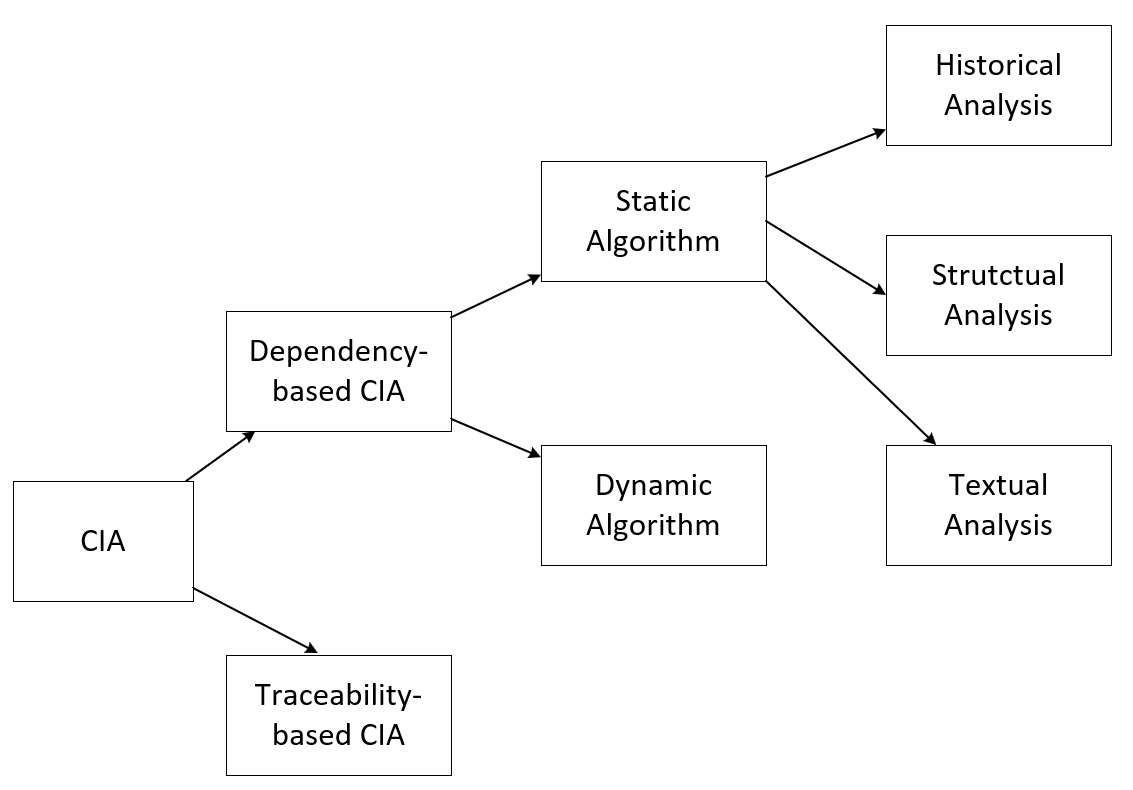
\includegraphics[scale=0.5]{CIA-hierarchy}
	\label{fig:cia-hierarchy}
	\caption{Các phương pháp CIA}
\end{figure}

Trong hơn 30 năm qua, đã có nhiều kỹ thuật CIA được nghiên cứu và đề xuất. Hình \ref{fig:cia-hierarchy} mô tả về các phương pháp CIA hiện nay đã được đề xuất. Một số phương pháp CIA dựa trên phân tích sự truy vết (traceability-based CIA) trong khi một số khác tập trung phân tích các mối quan hệ phụ thuộc (dependency-based CIA) để xác định các ảnh hưởng. Traceability-based CIA sẽ cố gắng truy vết mối liên kết giữa các phần tử trong từng mức trừu tượng với các thành phần tương ứng ở các mức khác (các mức trừu tượng: yêu cầu, tài liệu đặc tả, thiết kế, mã nguồn, ca kiểm thử). Mục tiêu của nó là gắn kết các thể hiện ở mỗi mức trừu tượng khác nhau của các đối tượng phần mềm (ví dụ: tài liệu thiết kế với mã nguồn). Trong khi đó, Depedency-based CIA tập trung xác định các mối quan hệ phụ thuộc của các thành phần trong cùng một mức trừu tượng (ví dụ: mối quan hệ giữa các lớp, phương thức, thuộc tính trong mã nguồn). Depedency-based CIA thường được áp dụng ở mức trừu tượng chi tiết hơn Traceability-based CIA.

Để thực hiện Depedency-based CIA, ta có thể sử dụng hai phương pháp là phân tích tĩnh và động. Phân tích động sẽ yêu cầu thực thi ứng dụng, nó sẽ thu thập các thông tin trước, trong và sau khi chạy để xác định các mối quan hệ phụ thuộc. Phương pháp này mang lại chính xác cao nhưng đòi hỏi sự phức tạp và tốn kém. Bên cạnh đó, các phương pháp phân tích tĩnh dễ thực hiện và ít tốn kém. Chúng tập được thực hiện ngay trên mã nguồn phần mềm. Có thể chia các phương pháp tĩnh này thành ba loại chính: Phân tích dựa trên lịch sử được thực hiện bằng cách khai phá thông tin từ nhiều phiên bản tiến hóa của phần mềm, phương pháp thường cho nhiều kết quả dự đoán nhầm, nhiều phần tử ảnh hưởng dự đoán thật sự không bị ảnh hưởng; Phân tích ngữ nghĩa dựa trên việc trích xuất thông tin từ việc phân tích nội dung comment hoặc các định danh (ví dụ: tên biến, phương thức); Nổi trội nhất trong đó là phân tích cấu trúc, phương pháp này tập trung phân tích tĩnh cấu trúc của chương trình, xác định các mối quan hệ giữa các thành phần và xây dựng đồ thị phụ thuộc.

\section{Quy trình phân tích ảnh hưởng sự thay đổi}
\begin{figure}[h]
	\centering
	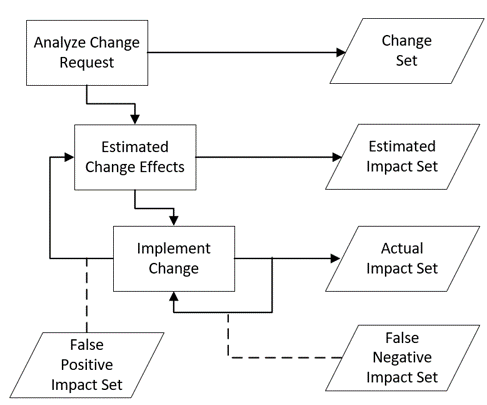
\includegraphics[scale=0.8]{CIA-process}
	\label{fig:cia-process}
	\caption{Quy trình chung CIA}
\end{figure}

Các loại thay đổi trong mã nguồn có thể chia làm hai loại chính là thay đổi cấu trúc và thay đổi lô-gíc. Thay đổi cấu trúc là các thay đổi liên quan đến các thành phần trong mã nguồn. Cụ thể đối với ngôn ngữ Java, thay đổi cấu trúc có thể là thay đổi về phạm vi truy cập, kiểu, tên của một thuộc tính hoặc thay đổi chữ kí của một phương thức. Thay đổi lô-gíc là thay đổi về thuật toán, các câu lệnh. Chúng thường là những thay đổi nằm trong thân phương thức.

Một thay đổi được thực hiện có thể gây ảnh hưởng không mong muốn đến những thành phần mã nguồn khác. Mục tiêu của các kỹ thuật CIA là xác định những thành phần ảnh hưởng. Hình \ref{fig:cia-process} thể hiện toàn bộ quy trình CIA. Phân tích ảnh hưởng sự thay đổi được bắt đầu bằng việc phân tích yêu cầu thay đổi để xác định được tập các thành phần thay đổi (Change Set - CS). Thông qua thuật toán CIA, các thành phần ảnh hưởng sẽ được phán đoán (Estimated Impact Set - EIS). EIS chính là đầu ra cuối cùng của quá trình CIA.

Phương pháp CIA hiệu quả là phương pháp giúp tìm ra được tập ảnh hưởng dự đoán gần nhất với tập ảnh hưởng thực tế khi thực hiện thay đổi (Actual Impact Set - AIS). Khi so sánh giữa EIS và AIS ta, có tập các thành phần ảnh hưởng tiên đoán nhầm (False Negative Impact Set - FNIS) và tập các thành phần ảnh hưởng tiên đoán thiếu (False Positive Impact Set - FPIS). Để đánh giá sự hiệu quả của một phương pháp CIA, người ta dùng hai độ đo là độ chính xác (Precision - P) và Recall - R, được tính theo các công thức \ref{exp:cia-precision} và \ref{exp:cia-recall}. Độ chính xác càng cao, tập FNIS sẽ càng bé, ta ít phải chú ý đến những thành phần không cần thiết. Độ hồi tưởng càng cao, tập FPIS càng bé, giúp ta phát hiện nhiều thành phần bị ảnh hưởng hơn giúp giảm số lỗi tiềm ẩn sau khi áp dụng phương pháp CIA.

\begin{equation}
	Precision = \frac{|EIS \cap AIS|}{EIS}
	\label{exp:cia-precision}
\end{equation}
\\
\begin{equation}
	Recall = \frac{|EIS \cap AIS|}{AIS}
	\label{exp:cia-recall}
\end{equation}

\newpage
\chapter{Phân tích ảnh hưởng sự thay đổi cho các ứng dụng J2EE}
\section{Tiền xử lý mã nguồn ứng dụng J2EE}
\textbf{Định nghĩa:} (\textit{Cây cấu trúc}) Cho mã nguồn ứng dụng J2EE, một cây cấu trúc của mã nguồn này được định nghĩa $T = (N, R)$ với $N = \{n_1, n_2,..., n_k\}$ là tập nút đại diện cho các thành phần trong mã nguồn như thư mục; tệp; lớp, phương thức, thuộc tính (Java); thẻ (XML-based); v,v. $R = \{(n_i, n_j) | n_i,n_j \in N\}$ là tập các cạnh. Mỗi cạnh $(r_i,r_j)$ đại diện cho quan hệ phụ thuộc giữa $n_i$ và $n_j$ có nghĩa là $n_i$ phụ thuộc vào $n_j$.

Các ứng dụng doanh nghiệp J2EE, ngoài sử dụng mã nguồn Java còn nhiều định dạng mã nguồn khác để đảm nhiệm vai trò cho tầng \textit{View} và các thành phần cấu hình ứng dụng như XML, JSP, XHTML, FreeMarker,...Với mỗi một định dạng lại có cấu trúc và cú pháp khác nhau, tuy nhiên ta có thể phân loại thành hai nhóm là mã nguồn Java và mã nguồn XML-based (mã nguồn có cú pháp dựa trên định dạng XML). Bộ tiền xử lý cần biến đổi những mã nguồn này về định dạng chung là cây cấu trúc, các nút trên cây cấu trúc cần chứa những thông tin cần thiết cho việc phân tích phụ thuộc cũng như cây cần được thiết kế để tối ưu cho việc duyệt và tìm kiếm các nút trên cây dễ dàng.

\subsection{Tiền xử lý cho mã nguồn Java và mã nguồn định dạng XML}
Hình \ref{fig:preprocess} thể hiện phương pháp để tiền xử lý mã nguồn ứng dựng J2EE. Hai phương pháp chính được đề xuất để thực hiện tiền xử lý cho mã nguồn Java và mã nguồn XML-based. Một phương pháp duyệt thư mục cũng cần được đề xuất và thực hiện nhằm tìm ra các tệp chứa mã nguồn Java và XML-based trong mã nguồn ứng dụng.

\begin{figure}[h]
	\centering
	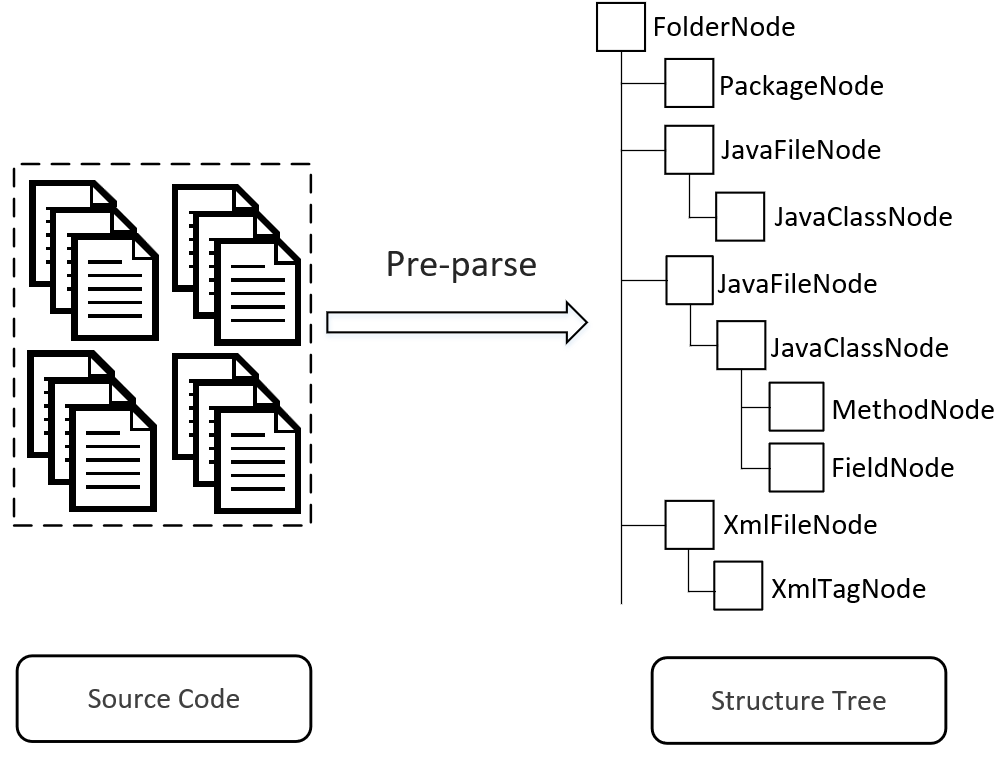
\includegraphics[scale=0.5]{preprocess}
	\label{fig:preprocess}
	\caption{Phương pháp tiền xử lý mã nguồn}
\end{figure}

Đầu tiên, ta thực hiện duyệt toàn bộ cấu trúc các thư mục và tệp trong mã nguồn ứng dụng. Ta có thể sinh được cây cấu trúc cơ bản gồm các nút thư mục và nút tệp. Tiếp theo, ta duyệt tìm tất cả các nút tệp trên cây. Các tệp mã nguồn có phần mở rộng \textit{.java} sẽ được phân tích  để thu thập thông tin và tạo các nút con tương ứng với các thành phần mã nguồn Java đó (lớp, thuộc tính, phương thức). Các thông tin của các thành phần này cũng cần được thu thập (ví dụ: đối với phương thức cần thu thập thông tin về kiểu trả về, mức truy cập, tên phương thức, danh sách các tham số). Hiện nay có một thư viện mã nguồn mở Java có tên Java Development Tools \footnote{https://www.eclipse.org/jdt/} đã hỗ trợ việc phân tích và thu thập thông tin cho các tệp mã nguồn Java. Tuy nhiên đầu ra của thư viện này chứa khá nhiều thông tin không cần thiết. Ta chỉ cần trích xuất những thông tin cần thiết để thêm vào cây cấu trúc. Các tệp mã nguồn có phần mở rộng \textit{.xml, .jsp, .html} sẽ xử lý bởi cùng một phương pháp tiền xử lý cho định dạng mã nguồn dựa trên XML. Kết quả đầu ra sẽ là các nút tương ứng với các thẻ XML có trong tệp. Các nút này cũng cần chứa toàn bộ thông tin của thẻ đấy, bao gồm các thuộc tính và nội dung của thẻ.

\subsection{Định danh các nút trên cây cấu trúc}
Cây cấu trúc là dữ liệu được sử dụng xuyên suốt trong các quá trình phân tích. Sẽ có rất nhiều hoạt động phân tích cần đến việc tìm kiếm và truy xuất dữ liệu của các nút trên cây. Vì thế việc định danh cho các nút trên cây là một việc rất quan trọng. Phương pháp đề xuất là định danh bằng đường dẫn tuyệt đối của nút. Đường dẫn tuyệt đối của mỗi nút trên cây sẽ được tạo thành bởi tên lần lượt của các nút cha và tên của nó, ngăn cách bởi kí tự gạch chéo (\texttt{/}). Với hầu hết các nút đại diện trong thành phần mã nguồn sẽ có đường dẫn tuyệt đối duy nhất, ta có thể thực hiện \textit{Indexing} các nút trên cây phục vụ cho việc tìm kiếm nhanh. Tuy nhiên, trong một số trường hợp, dùng tên các nút để tạo thành đường dẫn tuyệt đối sẽ có thể cho cùng một kết quả đối với nhiều hơn một nút.

\begin{lstlisting}[language=Java,
caption={Ví dụ chồng hàm trong Java},label={code:java-overloading}]
package vn.sample.manager.BookManager;
import vn.sample.model.Boook;
import vn.sample.model.Author;
public class BookManager {
	//...	
	public void addBook(Book newBook) {
		//...
	}
	public void addBook(String bookName, Author author) {
		//...
	}
}
\end{lstlisting}

Ví dụ như ở Mã nguồn \ref{code:java-overloading} thể hiện sự chồng hàm của phương thức \texttt{addBook()}. Nếu chỉ sử dụng tên của phương thức thì ta sẽ không định danh cho các các nút tương ứng với hai phương thức này được. Do vậy ta cần sử dụng cả thông tin về các tham số của chúng để tạo đường dẫn tuyệt đối. Bao gồm cả tên, kiểu và thứ tự của các tham số này trong phần khai báo phương thức. Kết quả ta được hai đường dẫn tuyệt đối có thể đại diện cho sự riêng biệt của các nút phương thức Java này.

\begin{verbatim}
vn/sample/manager/BookManager.java/BookManager/
addBook(vn.sample.model.Book_newBook)

vn/sample/manager/BookManager.java/BookManager/
addBook(java.lang.String_bookName,java.lang.String_author)
\end{verbatim}

Hoặc đối với mã nguồn dựa trên định dạng XML như ở Mã nguồn \ref{code:html-example}, nếu dùng tên thẻ để làm đường dẫn tuyệt đối thì hai phần tử \texttt{h1} sẽ có chung giá trị là \texttt{web/hello.html/html/body/h1}. Để định danh cho hai phần này, ta sẽ dùng thêm các thuộc tích đặc biệt là tọa độ thẻ mở của chúng trong mã nguồn. Ví dụ với phần \texttt{h1} đầu tiên, sẽ có tọa độ số dòng là 3, số cột là 12 cho nên đường dẫn tuyệt đối của nó sẽ là \texttt{web/hello.html/html/body/h1:3:12}. Đường dẫn mới này sẽ giúp phân biệt phần tử này với phần liền kề với đường dẫn \texttt{web/hello.html/html/body/h1:4:12}. Thật may mắn nền tảng Java cung cấp sẵn một thư viện giúp chúng ta phân tích các tệp có định dạng XML và lấy được tọa độ của các phần tử này. SAXParser sẽ giúp ta tiết kiệm công sức rất nhiều trong việc tiền xử lý phần mã nguồn này.

\begin{lstlisting}[language=XML,
caption={Ví dụ mã nguồn HTML},label={code:html-example}]
<html>
	<body>
		<h1>Hello!</h1>
		<h1>I am writing this line with Latex.</h1>
	</body>
</html>
\end{lstlisting}

\section{Phân tích phụ thuộc Struts}
\subsection{Giới thiệu mô hình kiến trúc Struts}
Apache Struts (trước đây được gọi là Struts2 để phân biệt với Struts1) là một trong những framework được ưa chuộng nhất để phát triển các ứng dụng web J2EE. Tương tự Spring MVC, Struts tuân theo mô hình xử lý MVC mà bản thân nó chứa đủ các thành phần giúp lập trình viên định nghĩa rõ ràng các thành phần Model, View và Controller.

\begin{figure}[h]
	\centering
	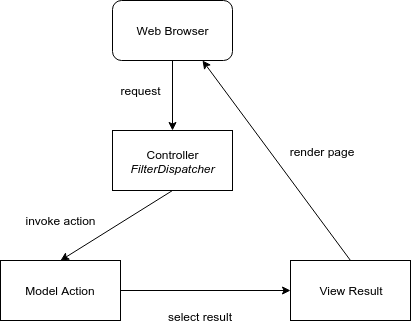
\includegraphics[scale=0.8]{struts-architecture}
	\label{fig:struts-architecture}
	\caption{Mô hình thiết kế của ứng dụng Struts}
\end{figure}

Hình \ref{fig:struts-architecture} thể hiện mô hình thiết kế của một ứng dụng Struts. Các thành phần chính của nó được thiết kế tương ứng với các phần trong mô hình MVC chung.

\textbf{Model:} là các lớp Java định nghĩa các đối tượng để chứa dữ liệu (POJO). Chúng chỉ đơn thuần có phương thức getter/setter tương ứng với các thuộc tính.

\textbf{View:} là các tệp JSP, dùng để hiển thị dữ liệu tới người dùng. Việc lấy dữ liệu từ Model để hiển thị lên View được thực hiện nhờ một thành phần trong Struts có tên là OGNL (Object-graph Navigation Language).

\textbf{Controller:} là phần xử lý lô-gíc, trong Struts được gọi là Action. Mỗi Action sẽ là một lớp Java, thường kế thừa từ lớp \textit{ActionSupport} của Struts. Trong lớp Action này có chứa tham chiếu đến lớp Java của phần Model, từ đó có thể dễ dàng truy cập dữ liệu từ phần Model. Các phương thức bên trong lớp Action sẽ thực hiện truy xuất và xử lý dữ liệu từ lớp Model. Sau khi thực hiện xử lý xong, phương này có thể cập nhật lại dữ liệu và chuyển hướng đến một View tương ứng để hiển thị kết quả tới người dùng.

\subsection{Làm mịn cây cấu trúc}

\subsection{Phân tích tệp cấu hình Struts}
Thông thường một ứng dụng Struts sẽ có một tệp cấu hình chính có tên là \textit{struts.xml}. Tại đây, chúng ta có thể dễ dàng thu thập được các thông tin về toàn bộ các thành phần trong ứng dụng được khai báo: bao gồm các Action và View Results. Để xác định các mối quan hệ phụ thuộc giữa các thành phần Struts, tệp cấu hình chính là điểm bắt đầu để phân tích. Tệp cấu hình này đã được làm mịn ở bước tiền xử lý mã nguồn, cho ta thông tin về các Package, Action, Result, Interceptor, ResultType - những đối tượng của Struts.

\section{Phương pháp phân tích ảnh hưởng sự thay đổi WAVE-CIA}

\begin{figure}[h]
	\centering
	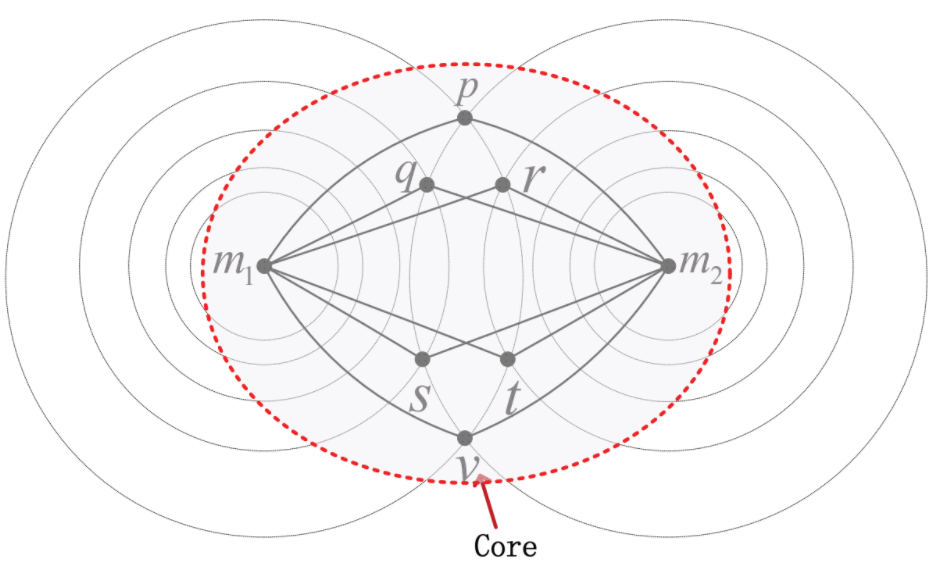
\includegraphics[scale=0.5]{wave-cia-phenomenon}
	\label{wave-cia-phenomenon}
	\caption{Hiện tượng lan truyền sóng nước trên đồ thị gọi}
\end{figure}

Trong việc xây dựng công cụ này, WAVE-CIA được sử dụng làm phương pháp phân tích ảnh hưởng sự thay đổi. WAVE-CIA là một phương pháp phân tích tĩnh trực tiếp trên mã nguồn ứng dụng, sử dụng một bản biểu diễn chương trình dưới dạng đồ thị gọi (Call Graph - CG) tĩnh. Ý tưởng của phương pháp này dựa trên sự mô phỏng hiện tượng lan truyền sóng nước, được mô tả như Hình \ref{wave-cia-phenomenon}. Hầu hết các phương pháp CIA đưa ra dự đoán tập ảnh hưởng dựa trên từng thành phần riêng lẻ của tập thay đổi chứ không xem xét mối quan hệ giữa chúng. Trong khi đó, nhiều thay đổi có thể được thực hiện cùng lúc để đáp ứng một yêu cầu thay đổi nào đó. WAVE-CIA dựa trên nguyên tắc này, và nó có thể dự đoán tập ảnh hưởng tốt hơn với tập thay đổi gồm nhiều phần tử.

Để thực hiện phương pháp này, một đồ thị gọi cần được xây dựng đầu tiên. Sau đó, những phần tử tập cốt lõi sẽ được tìm ra, tập ảnh hưởng cuối cùng sẽ được tính toán dựa vào tập cốt lõi.

\subsection{Xây dựng đồ thị gọi}
Đồ thị gọi là một đồ thị có hướng $G = (V, E)$. $V$ là tập các đỉnh tương ứng với các nút trong cây cấu trúc (lớp, phương thức, thuộc tính Java; phần tử XML; tệp JSP, HTML), và $E \subseteq V \times V$ là tập các cạnh biểu diễn cho các mối quan hệ phụ thuộc giữa các nút này.

Để xây dựng được đồ thị gọi cho phương pháp CIA, ta chỉ cần chuyển đổi từ cây cấu trúc. Các bước để thực hiện được trình bày ở Thuật toán \ref{algo:build-call-graph}.

\begin{thuattoan}
	\label{algo:build-call-graph}
	\caption{Xây dựng đồ thị gọi từ cây cấu trúc}
	\SetKwInOut{Input}{Input}
	\SetKwInOut{Output}{Output}
	\SetKwInOut{Use}{Use}
	\Input{$T = (N, R)$ là cây cấu trúc của ứng dụng}
	\Output{$G = (V, E)$ là đồ thị gọi của ứng dụng}
	\Use{$getCallees(n)$ là các nút được gọi hoặc sử dụng bởi $n$}
	V = $\emptyset$, E = $\emptyset$\;
	\ForEach{$n \in N$}{
		$V = V \cup \{n\}$\; 
		\ForEach{$ne \in getCallees(n)$} {$E = E \cup (n, ne)$\;}
	} 
	\Return V\;
\end{thuattoan}

\subsection{Xác định tập cốt lõi}
Như đã nói ở trên, hầu hết các phương pháp CIA hiện nay tính toán tập ảnh hưởng mà không quan tâm đến mối quan hệ của các phần tử trong tập thay đổi. Trong thực tế, luôn có mối quan hệ giữa các phần tử trong tập thay đổi. Chúng ta sẽ sử dụng hiện tượng này trong việc ước tính tập ảnh hưởng. Đầu tiên ta cần tìm tập cốt lõi, nó là tập gồm các thành phần thường bị ảnh hưởng bởi nhiều phần tử trong tập thay đổi nhất. Việc tính toán tập cốt lõi được thực hiện bằng việc khai thác thông tin từ đồ thị gọi, các bước thực hiện như Thuật toán \ref{algo:cal-core-set}.

\begin{thuattoan}
	\label{algo:cal-core-set}
	\caption{Xác định tập cốt lõi}
	\SetKwInOut{Input}{Input}
	\SetKwInOut{Output}{Output}
	\SetKwInOut{Use}{Use}
	\Input{
		$G = (V, E)$ là đồ thị gọi của ứng dụng\\
		$CS$ gồm những phần tử của tệp thay đổi\\
		$depth$ là độ sâu tìm kiếm
	}
	\Output{$Core$ là tập cốt lõi}
	\Use{$getNeighborSet(m, depth)$ là tập các đỉnh có quan hệ với đỉnh $m$ với khoảng cách $depth$}
	
	$tempSet = \emptyset$\;
	\ForEach{$v \in V$}{
		$neighborSet = getNeighborSet(m, depth)$\;
		$neighborCSSet = neighborSet \cap CS$\;
		\If{$|neighborSet| > 1$} {$tempSet = tempSet \cup \{m\}$}
	}
	$Core = CS \cup tempSet$\;
	\Return $Core$\;
\end{thuattoan}

Các phần tử trong tập cốt lõi được định nghĩa là các đỉnh \textit{láng giềng} với nhiều hơn một phần tử trong tập thay đổi. \textit{Láng giềng} tức là có quan hệ phụ thuộc giữa hai đỉnh trên đồ thị gọi nhỏ hơn một khoảng cách $depth$ cho trước. Khoảng cách $depth$ sẽ thay đổi với từng bài toán để cân bằng giữa độ chính xác và độ hồi tưởng của phương pháp để phù với từng loại yêu cầu cụ thể (ví dụ: cần độ chính xác cao thay vì quan tâm đến độ hồi tưởng cao).

\subsection{Tính toán tập ảnh hưởng}
Mặc dù tập cốt lõi có thể cho kết quả có độ chính xác tốt nhờ vào điều chỉnh $depth$, tuy vẫn có những phần tử bị dự đoán ảnh hưởng thiếu (thực tế phần tử đó bị ảnh hưởng nhưng không xuất hiện trong tập cốt lõi). Do vậy ta cần tính toán để tìm thêm các phần tử còn sót này, ta sẽ mở rộng tập cốt lõi để xây dựng tập ảnh hưởng cuối cùng (Final Impact Set - FIS) nhằm tăng độ hồi tưởng cho phương pháp. Phương pháp tính toán FIS được thể hiện như Thuật toán \ref{algo:cal-fis}.

\begin{thuattoan}
	\label{algo:cal-fis}
	\caption{Tính toán tập ảnh hưởng}
	\SetKwInOut{Input}{Input}
	\SetKwInOut{Output}{Output}
	\SetKwInOut{Use}{Use}
	\Input{
		$G = (V, E)$ là đồ thị gọi của ứng dụng\\
		$Core$ là tập cốt lõi\\
	}
	\Output{$FIS$ là tập ảnh hưởng}
	\Use{$getCallerSet(m, depth)$ là tập các đỉnh gọi hoặc sử dụng $m$ trong khoảng cách $depth$\\
		$getCalleeSet(m, depth)$ là tập các đỉnh được gọi hoặc sử dụng bởi $m$ trong khoảng cách $depth$\\}
	
	
	$FIS = Core$\;
	\While{$FIS$ có số lượng phần tử không ổn định} {
		\ForEach{$v \in V$}{
			\If{$m \notin FIS$}{
				$callerSet = getCallerSet(v)$\;
				$calleeSet = getCalleeSet(v)$\;
				\If{$FIS \cap callerSet \neq \emptyset \wedge FIS \cap calleeSet \neq \emptyset$}{
					$FIS = FIS \cup \{v\}$
				}
			}
		}
	}
	
	\Return $FIS$\;
\end{thuattoan}

Một phần tử $v$ sẽ được thêm vào tập ảnh hưởng nếu $v$ thỏa mãn điều kiện khi $v$ được gọi hoặc sử dụng bởi $v_1$ và $v_2$, hoặc ngượi lại $v_1$ và $v_2$ gọi hoặc sử dụng $v$; trong khi $v_1$ và $v_2$ là hai phần tử thuộc tập cốt lõi. Sau khi duyệt tất cả các phần tử, tập ảnh hưởng có thể được sử dụng tiếp như tập cốt lõi để tiếp tục mở rộng tập ảnh hưởng nếu nó chưa đủ tốt để tăng độ phủ cho phương pháp. Thuật toán có thể dừng lại khi kích thước tập ảnh hưởng đạt mức ổn định.

\chapter{Quản lý các phiên bản}
Các nhà bảo trì phần mềm cần phải hiểu về ứng dụng phần mềm trước khi thực hiện các sửa đổi trên nó. Mặc dù mã nguồn hệ thống thường được xem xét (review) cẩn thận, tuy nhiên chỉ xem xét cho mã nguồn ở phiên bản hiện tại là không đủ để hiểu rõ sự tiến hóa của nó. Các nhà bảo trì cũng nên hiểu được mã nguồn đã được thay đổi như thế nào trước đó.

Quản lý phiên bản là công việc lưu trữ các thay đổi của ứng dụng phần mềm theo thời gian, nó có thể giúp ta theo dõi các thay đổi qua thời phát triển, bảo trì và hoàn toàn có thể khôi phục lại một phiên bản xác định nào đó sau này. Một số hệ thống quản lý phiên bản phổ biến hiện nay như Git \footnote{https://git-scm.com} hay SVN  \footnote{https://subversion.apache.org} tập trung lưu trữ các thay đổi ở mức các dòng mã nguồn. Các hệ thống này có thể trích xuất thông tin về sự khác nhau giữa các lần sửa đổi của một tệp mã nguồn được lưu trữ. Một tập hợp các thông tin này được xem như là lịch sử thay đổi của tệp mã nguồn đấy.

Tuy nhiên, trong thực tế có một vài bất lợi cho các nhà bảo trì khi sử dụng các hệ thống này để theo dõi lịch sử thay đổi của ứng dụng phần mềm. Ở mỗi lần cam kết (commit - xác nhận lưu trữ thay đổi), lập trình viên thường sửa đổi rất nhiều thứ xen kẽ nhau chứ không chỉ thực hiện một thay đổi. Các công cụ phát hiện ở mức dòng mã nguồn khó tách rời những thay đổi này ra và phát hiện riêng rẽ từng thay đổi trong một lần cam kết đấy. Nếu các nhà bảo trì phải thực hiện công việc này bằng tay, nó sẽ tốn rất nhiều thời gian và chi phí.

Để giải quyết vấn đề nhiều thay đổi xuất hiện xen kẽ trong cùng một lần cam kết. Một hướng tiếp cận để phát hiện thay đổi mới được để xuất. Cơ chế này sẽ phát hiện thay đổi trên một dạng dữ liệu trừu tượng là cây cấu trúc của các phiên bản ứng dụng chứ không phải những dòng mã nguồn. Trong các chương trình hướng đối tượng như J2EE, các lớp, phương thức, thuộc tính sẽ thích hợp làm đơn vị cho các thay đổi. Việc sử dụng cây cấu trúc làm dữ liệu để thực hiện phát hiện thay đổi so với dòng mã giúp trừu tượng hóa các thay đổi, giảm lượng thông tin cần xử lý cho người bảo trì nhưng vẫn cung cấp đủ thông tin để họ có thể hiểu sự tiến hóa của ứng dụng. Ngoài việc cung cấp đầu vào cho việc lưu trữ thay đổi, cơ chế so sánh này còn giúp ích trong việc tự động thực hiện phân tích ảnh hưởng sự thay đổi. Các thành phần mã nguồn thay đổi được thu thập từ bộ so sánh được sử dụng làm tập thay đổi cho thuật toán CIA.

\section{Phát hiện thay đổi cho mã nguồn Java}
Các thành phần mã nguồn Java có thể chia làm ba loại chính gồm lớp, phương thức và thuộc tính. Có rất nhiều loại thay đổi đối với những thành phần mã nguồn này, ví dụ như mở rộng mức truy cập từ \textit{private} thành \textit{public}, thay đổi lớp cha đối với lớp hoặc thay đổi tham số đối với phương thức, v.v. Tất cả các loại thay đổi cho Java được liệt kê ở các Bảng \ref{tbl:field-ct} và Bảng \ref{tbl:class-method-changes}.


\begin{table}[h]
	\centering
	\caption{Các loại thay đổi của thuộc tính Java}
	\label{tbl:field-ct}
	\begin{tabular}{|l|l|}
		\hline
		\textbf{Kí hiệu} & \textbf{Ý nghĩa}                                        \\ \hline
		AF               & Thêm thuộc tính mới                                            \\ \hline
		DF               & Xóa thuộc tính                                                 \\
		\hline
		CNF               & Đổi tên thuộc tính                                                 \\
		\hline
		IAF              & Mở rộng mức truy cập của thuộc tính                            \\ \hline
		DAF              & Thu hẹp mức truy cập của thuộc tính                            \\ \hline
		AFF              & Thêm từ khóa \textit{final} cho thuộc tính    \\ \hline
		DFF              & Xóa từ khóa \textit{final} của thuộc tính     \\ \hline
		ASF              & Thêm từ khóa \textit{static} cho thuộc tính   \\ \hline
		DSF              & Xóa từ khóa \textit{static} của thuộc tính    \\ \hline
		CSF              & Thay đổi kiểu của thuộc tính    \\ \hline
	\end{tabular}
\end{table}

\begin{table}[h]
	\centering
	\caption{Các loại thay đổi của lớp và phương thức Java}
	\label{tbl:class-method-changes}
	\begin{tabular}{|l|p{6cm}|l|p{6cm}|}
		\hline
		\textbf{Kí hiệu} & \textbf{Ý nghĩa}                                        & \textbf{Kí hiệu} & \textbf{Ý nghĩa}                                                \\ \hline
		\multicolumn{2}{|l|}{\textit{Các loại thay đổi của lớp}}                   & \multicolumn{2}{l|}{\textit{Các loại thay đổi của phương thức}}                    \\ \hline
		AC               & Thêm lớp mới                                            & AM               & Thêm phương thức mới                                            \\ \hline
		DC               & Xóa lớp                                                 & DM               & Xóa phương thức                                                 \\ \hline
		CNC              & Đổi tên lớp                                             & CNM              & Đổi tên phương thức                                             \\ \hline
		IAC              & Mở rộng mức truy cập của lớp                            & IAM              & Mở rộng mức truy cập của phương thức                            \\ \hline
		DAC              & Thu hẹp mức truy cập của lớp                            & DAM              & Thu hẹp mức truy cập của phương thức                            \\ \hline
		AFC              & Thêm từ khóa \textit{final} cho lớp    & AFM              & Thêm từ khóa \textit{final} cho phương thức    \\ \hline
		DFC              & Xóa từ khóa \textit{final} của lớp     & DFM              & Xóa từ khóa \textit{final} của phương thức     \\ \hline
		ASC              & Thêm từ khóa \textit{static} cho lớp   & ASM              & Thêm từ khóa \textit{static} cho phương thức   \\ \hline
		DSC              & Xóa từ khóa \textit{static} của lớp    & DSM              & Xóa từ khóa \textit{static} của phương thức    \\ \hline
		AAbC             & Thêm từ khóa \textit{abstract} cho lớp & AAbM             & Thêm từ khóa \textit{abstract} cho phương thức \\ \hline
		DAbC             & Xóa từ khóa \textit{abstract} của lớp  & DAbM             & Xóa từ khóa \textit{abstract} của phương thức  \\ \hline
		APC              & Thêm lớp cha                                            & CM               & Thay đổi nội dung thân phương thức                              \\ \hline
		DPC              & Xóa lớp cha                                             & CRM              & Thay đổi kiểu trả về của phương thức                            \\ \hline
		CPC              & Thay đổi lớp cha                                        & CPM              & Thay đổi danh sách tham số của phương thức                      \\ \hline
	\end{tabular}
\end{table}

\begin{thuattoan}
	\label{algo:class-change}
	\caption{$ClassChange(F_{t1}, F_{t2})$}
	\SetKwInOut{Input}{Input}
	\SetKwInOut{Output}{Output}
	\Input{$F_{t1}, F_{t2}$ lần lượt đại diện cho các nút của tệp chứa thay đổi ở phiên bản $t1$ và $t2$}
	\Output{$CS$ là danh sách các thay đổi}
	
	$C_{t1}$ = tất cả lớp trong $F_{t1}$\;
	$C_{t2}$ = tất cả lớp trong $F_{t2}$\;
	CS = $\emptyset$\;
	\ForEach{$c_1 \in C_{t1}, c_2 \in C_{t2}$}{
		\If{$c_1.name = c_2.name$}{
			$CS = CS \cup compareFinalModifier(c_1, c_2)$\;
			$CS = CS \cup compareVisibilityModifier(c_1, c_2)$\;
			$CS = CS \cup compareStaticModifier(c_1, c_2)$\;
			$CS = CS \cup compareAbstractModifier(c_1, c_2)$\;
			\If{$c_1.parent = null \wedge c_2.parent \neq null$} {
				$CS = CS \cup (c_1, APC)$\;
			}\ElseIf{$c_1.parent \neq null \wedge c_2.parent = null$}{
				$CS = CS \cup (c_1, DPC)$\;
			}\ElseIf{$c_1.parent \neq null \wedge c_1.parent \neq c_2.parent$}{
				$CS = CS \cup (c_1, CPC)$\;
			}
			$CS = CS \cup FieldChange(c_1, c_2)$\;
			$CS = CS \cup MethodChange(c_1, c_2)$\;
			$C_{t1} = C_{t1} \setminus \{c_1\}$\;
			$C_{t2} = C_{t2} \setminus \{c_2\}$\;
		}
	}
	\ForEach{$c_1 \in C_{t1}$}{
		$CS = CS \cup (c_1, DC)$\;
	}
	\ForEach{$c_2 \in C_{t2}$}{
		$CS = CS \cup (c_1, AC)$\;
	}
	\Return $CS$\;
\end{thuattoan}

Để so phát hiện sự thay đổi của các lớp Java, các bước thực hiện như Thuật toán \ref{algo:class-change}. Đầu tiên, ta cần thu thập tất cả danh sách các lớp này của tệp thay đổi (từ $F_{t1}$ thành $F_{t2}$). Duyệt lần lượt các phần tử trong danh sách lớp ở phiên bản $t1$ từng đôi một với các phần tử ở phiên bản $t_2$. Đối với những cặp phần tử nào có tên lớp giống nhau, ta thực hiện so sánh các thuộc tính của chúng bao gồm: từ khóa $final$, từ khóa $static$, từ khóa $abstract$ và mức truy cập của lớp. Ngoài ra ta cũng cần so sánh về khai báo lớp cha của các phần tử. Nếu ở phiên bản $t1$ phần tử chưa có lớp cha mà phiên bản $t2$ có thì đây là kiểu thay đổi \textbf{APC} và ngược lại ở phiên bản $t1$ có nhưng $t2$ không có thì là \textbf{DPC}. Còn nếu trong trường hợp cả hai phiên bản đều có lớp cha nhưng tên của lớp cha này là khác nhau thì đây là kiểu thay đổi \textbf{CPC}. Ở những phần tử có tên giống nhau, ta cũng thực hiện gọi các phương thức để so sánh các thuộc tính và phương thức của chúng $FieldChange()$, $MethodChange()$ để tìm ra những thay đổi ở các thành còn của phần tử này. Sau khi duyệt xong, những phần tử thuộc danh sách phiên bản $t1$ là các phần đã bị xóa đi cho nên kiểu thay đổi là \textbf{DC}, các phần tử thuộc danh sách phiên bản $t2$ tương tự là những phần tử mới có kiểu thay đổi là \textbf{AC}.

\begin{thuattoan}
	\label{algo:field-change}
	\caption{$FieldChange(C_{t1}, C_{t2})$}
	\SetKwInOut{Input}{Input}
	\SetKwInOut{Output}{Output}
	\Input{$C_{t1}, C_{t2}$ lần lượt đại diện cho các nút của lớp chứa thay đổi ở phiên bản $t1$ và $t2$}
	\Output{$CS$ là danh sách các thay đổi}
	
	$F_{t1}$ = tất cả thuộc tính trong $C_{t1}$\;
	$F_{t2}$ = tất cả thuộc tính trong $C_{t2}$\;
	CS = $\emptyset$\;
	\ForEach{$f_1 \in F_{t1}, f_2 \in F_{t2}$}{
		\If{$f_1.name = f_2.name$}{
			$CS = CS \cup compareFinalModifier(f_1, f_2)$\;
			$CS = CS \cup compareVisibilityModifier(f_1, f_2)$\;
			$CS = CS \cup compareStaticModifier(f_1, f_2)$\;
			\If{$f_1.type \neq f_2.type$} {
				$CS = CS \cup (f_1, CSF)$\;
			}
			$F_{t1} = F_{t1} \setminus \{f_1\}$\;
			$F_{t2} = F_{t2} \setminus \{f_2\}$\;
		}
	}
	\ForEach{$f_1 \in F_{t1}$}{
		$CS = CS \cup (f_1, DF)$\;
	}
	\ForEach{$f_2 \in F_{t2}$}{
		$CS = CS \cup (f_1, AF)$\;
	}
	\Return $CS$\;
\end{thuattoan}

\begin{thuattoan}
	\label{algo:method-change}
	\caption{$MethodChange(C_{t1}, C_{t2})$}
	\SetKwInOut{Input}{Input}
	\SetKwInOut{Output}{Output}
	\Input{$C_{t1}, C_{t2}$ lần lượt đại diện cho các nút của lớp chứa thay đổi ở phiên bản $t1$ và $t2$}
	\Output{$CS$ là danh sách các thay đổi}
	
	$M_{t1}$ = tất cả phương thức trong $C_{t1}$\;
	$M_{t2}$ = tất cả phương thức trong $C_{t2}$\;
	CS = $\emptyset$\;
	\ForEach{$m_1 \in M_{t1}, m_2 \in M_{t2}$}{
		\If{$m_1.name = m_2.name$}{
			$CS = CS \cup compareFinalModifier(m_1, m_2)$\;
			$CS = CS \cup compareVisibilityModifier(m_1, m_2)$\;
			$CS = CS \cup compareStaticModifier(m_1, m_2)$\;
			$CS = CS \cup compareAbstractModifier(m_1, m_2)$\;
			\If{$m_1.returnType \neq m_2.returnType$} {
				$CS = CS \cup (m_1, CRM)$\;
			}
			\If{$m_1.body \neq m_2.body$} {
				$CS = CS \cup (m_1, CM)$\;
			}
			\If{$m_1.param \neq m_2.param$} {
				$CS = CS \cup (m_1, CPM)$\;
			}			
			$M_{t1} = M_{t1} \setminus \{m_1\}$\;
			$M_{t2} = M_{t2} \setminus \{m_2\}$\;
		}
	}
	\ForEach{$m_1 \in M_{t1}$}{
		$CS = CS \cup (m_1, DM)$\;
	}
	\ForEach{$m_2 \in M_{t2}$}{
		$CS = CS \cup (m_1, AM)$\;
	}
	\Return $CS$\;
\end{thuattoan}

Đối với phát hiện thay đổi cho thuộc tính và phương thức Java, các làm cũng tương tự so với lớp tuy nhiên sẽ đơn giản hơn như Thuật toán \ref{algo:field-change} và \ref{algo:method-change}. Đối với thuộc tính ta chỉ cần so sánh cho từ khóa $final$, $static$ còn phương thức thì thêm cả từ khóa $abstract$. Ngoài ra đối với thuộc tính ta cũng cần so sánh kiểu của nó để xác định loại thay đổi (\textbf{CSF}). Đối với phương thức, để tìm ra các loại thay đổi khác, ta cần so sánh kiểu trả về (\textbf{CRM}), thân phương thức (\textbf{DM}), danh sách tham số (\textbf{CPM}).

\chapter{Thực nghiệm và triển khai}
\section{Công cụ cài đặt}
Dựa trên những đề xuất phương pháp mới đã đề xuất trên đây. Bộ công cụ JCIA-VT, thừa kế mã nguồn từ JCIA, đã được triển khai và cài đặt sử dụng framework Spring trên nền tảng ứng dụng Web. Bộ công cụ này nhận đầu vào là toàn bộ mã nguồn dự án doanh nghiệp sử dụng các nền tảng và công nghệ J2EE dưới dạng tệp nén.

JCIA-VT gồm năm mô-đun chính: bộ xử lý cơ sở, bộ phân tích ảnh hưởng thay đổi, bộ phân tích cấu trúc, bộ trình diễn, bộ quản lý người dùng và lịch sử phân tích; chúng được thể hiện như Hình 3-1. Mô-đun xử lý cơ sở bao gồm hai thành phần con là bộ tiền xử lý mã nguồn và bộ phân tích phụ thuộc theo từng công nghệ để sinh cây cấu trúc và phụ thuộc cho các nút trên cây.

Trong bộ tiền xử lý, mã nguồn Java ban đầu được phân tích nhờ thư viện Java Development Tools (JDT)  hỗ trợ tới chuẩn JavaSE phiên bản 8; đối với mã nguồn XML, hai công cụ DOMParser và SAXParser của thư viện Java được sử dụng đồng thời để có được dữ liệu các thẻ XML theo cấu trúc cấp bậc cũng như tọa độ (số hàng, số cột) của từng thẻ để phục vụ cho yêu cầu định danh và tìm kiếm nút. Bộ phân tích ảnh hưởng thay đổi kế thừa từ công cụ JCIA, sử dụng và cải tiến kĩ thuật phân tích ảnh hưởng WAVE-CIA đã có; một bộ so sánh cũng được cài đặt để thực hiện nhiệm vụ so sánh hai phiên bản mã nguồn (trước và sau thay đổi) nhằm tìm ra các phần tử thay đổi kèm kiểu thay đổi của chúng để đưa vào thuật toán CIA. Mô-đun phân tích cấu trúc bao gồm năm chức năng nhiệm vụ chính là: phân tích kiến trúc công nghệ, xây dựng dòng dữ liệu, phân tích độ phức tạp của mã nguồn, dựng sơ đồ lớp và phân tích cơ sở dữ liệu. Phân tích kiến trúc công nghệ giúp người dùng nắm được công nghệ sử dụng tại dự án đầu vào, sự liên kết giữa các công nghệ giữa các tầng với nhau. Ví dụ: tại tầng liên kết cơ sở dữ liệu dự án sử dụng framework Hibernate kết nối tới hệ quản trị cơ sở dữ liệu MySQL tại tầng cơ sở dữ liệu. Bộ xây dựng dòng dữ liệu phân tích đường đi của dữ liệu từ thành phần này qua thành phần khác của dự án, cụ thể là từ thành phần giao diện đến các thành phần điều khiển và cuối cùng là cơ sở dữ liệu và ngược lại. Điều này cho phép người dùng hình dung được đường đi của dữ liệu trong dự án, giúp người quản lí có thể kiểm tra đối chiếu với bộ quy tắc lập trình, chia tầng ứng dụng của công ty. Bộ tính toán độ phức tạp của mã nguồn triển khai tính toán độ phức tạp của các lớp trong mã nguồn đầu vào dựa trên nhiều tiêu chí khác nhau. Từ đó, người dùng có thêm một góc nhìn đánh giá chất lượng mã nguồn nhằm đảm bảo về khả năng vận hành cũng như bảo trì, nâng cấp về giai đoạn sau của dự án. Bộ xây dựng sơ đồ lớp xây dựng sơ đồ lớp trong một gói và sơ đồ lớp của một lớp tùy thuộc vào mức độ mà người dùng kích hoạt từ giao diện. Sơ đồ lớp được xây dựng và hiển thị đúng theo chuẩn UML 2.0 giúp người dùng thấy được mối quan hệ giữa các lớp trong ứng dụng. Công cụ phân tích cơ sở dữ liệu thực hiện phân tích dựng lên cấu trúc cơ sở dữ liệu và phân tích phát hiện các thành phần tương tác với cơ sở dữ liệu. Công cụ này cho người dùng cái nhìn tổng quan về thiết kế cơ sở dữ liệu của dự án, phát hiện dòng dữ liệu đến cơ sở dữ liệu giúp hoàn thiện bộ phân tích dòng dữ liệu đã nêu trên. Vì là ứng dụng nền tảng Web, mô-đun trình diễn được phát triển với thư viện D3.js  kèm các API để hiển thị thông tin phân tích trực quan tới người dùng và giúp thực hiện các thao tác với hệ thống phía sau. Cuối cùng, với nhu cầu thực hiện phân tích nhiều mã nguồn cùng lúc, mô-đun quản lý người dùng và lịch sử phân tích cho phép nhiều người dùng sử dụng bộ công cụ cùng lúc và cho phép khôi phục lịch sử của các đợt phân tích từ trước.
\chapter{Kết luận}
Nghiên cứu này đã đề xuất các phương pháp và bộ công cụ phục vụ cho các hoạt động đảm bảo chất lượng mã nguồn các ứng dụng doanh nghiệp trên nền tảng và công nghệ J2EE. Ở giai đoạn này, chúng tôi đã hoàn thành cơ bản các chức năng chính của bộ công cụ nhằm đáp ứng cho việc phân tích mã nguồn các ứng dụng sử dụng Struts 2 và Hibernate. Dựa trên những gì đã thực hiện được, trong giai đoạn tiếp theo, sẽ có thêm nhiều phụ thuộc được thêm vào để xử lý giúp bộ phân tích ảnh hưởng dự đoán tập ảnh hưởng chính xác hơn. Bộ quản lý vào so sánh các phiên bản mã nguồn sẽ được tích hợp với các hệ thống quản lý phiên bản hiện nay như Git  và SVN . Điều này giúp cho việc thực hiện phân tích ảnh hưởng và báo cáo kết quả hoàn toàn tự động mà không cần đến các thao tác của con người. Đây cũng là một lợi thế để áp dụng các kĩ thuật CIA có tính chính xác cao hơn như kĩ thuật CIA dựa vào phân loại thay đổi bởi bộ so sánh phiên bản có thể xác định chính xác từng loại thay đổi trên các thành phần mã nguồn. Đối với các kiểm thử viên, chức năng phân tích ảnh hưởng có thể giúp họ chỉ cần thực hiện một số ca kiểm thử nhất định khi có đội phát triển thay đổi mã nguồn. Tuy nhiên, hiện nay hầu hết các ca kiểm thử được thực hiện dựa trên các tài liệu biên bản kiểm thử mà chúng mô tả các bước kiểm thử bằng tay trên giao diện ứng dụng chứ không phải tự động bằng Unit Test. Trong khi đó kết quả của bộ phân tích ảnh hưởng là các thành phần mã nguồn, do đó một bộ ánh xạ giữa thành phần mã nguồn và các màn hình hoặc chức năng ứng dụng cần được tích hợp để bộ công cụ này thực sự có ích và có thể ứng dụng đại trà vào quá trình đảm bảo chất lượng cho nền công nghiệp phát triển phần mềm ở các công ty hiện nay. Ngoài ra, cần có thêm nhiều góc nhìn về ứng dụng cần được tích hợp để người sử dụng thêm nhiều thông tin cho ứng dụng của mình như biểu đồ tuần tự giữa các package, biểu đồ dòng điều khiển và các công cụ đánh giá về độ phức tạp mã nguồn và bảo mật của ứng dụng, v.v. Bộ công cụ sẽ hỗ trợ cho thêm nhiều công nghệ và nền tảng khác của Java, và xa hơn nữa, nhóm sẽ nghiên cứu để bộ công cụ có thể phân tích cho các ngôn ngữ khác như C, PHP, Javascript.
\end{document}
